%%%%%%%%%%%%%%%%%%%%%%%%%%%%%%%
%%%%% LaTeX Template Basic %%%%
%%%%%% Version: 20230930 %%%%%%
%%%%%%%%% Author: YSQ %%%%%%%%%
%%%%%%%%%%%%%%%%%%%%%%%%%%%%%%%

%!TEX program = xelatex
\documentclass[12pt, a4paper]{article}

%%%%%%%%%%%%%%%%%%%%%%%%%%%%%%%
%%%%%% Package Including %%%%%%
%%%%%%%%%%%%%%%%%%%%%%%%%%%%%%%

%%%%%%%%%%%%% Math %%%%%%%%%%%%
\usepackage{amsmath, amsthm, amssymb}   % AMS Environment
\usepackage{yhmath} 					% Math symbols

%%%%%%%%%%%% Figure %%%%%%%%%%%
\usepackage{graphicx} 					% Graph including
%\graphicspath{{images/}} 				% Searching image directory 
%\usepackage{wrapfig} 					% Wrap figure 
%\usepackage{floatflt} 					% Float figure 
%\usepackage{subfig} 					% Subfigures
\usepackage{caption} 					% Captioning
\DeclareCaptionLabelFormat{bold}{\textbf{#1 #2}}
\captionsetup[figure]{labelformat=bold}
\captionsetup[table]{labelformat=bold}
\usepackage{lmodern}
\usepackage{diagbox} 					% Diagonal in table
\usepackage{tikz} 						% Graph drawing
%\usepackage{pgfplots} 					% Plotting

%%%%%%%%%%%%% Text %%%%%%%%%%%%
\usepackage{fontspec} 					% Font setting
\usepackage{type1cm} 					% Fontsize setting
\usepackage{titlesec} 					% Setting font of sections
%\usepackage{framed} 					% Font frames
%\usepackage{ulem} 						% Text decorating

%%%%%%%%%%%% Others %%%%%%%%%%%
\usepackage{fancyhdr} 					% Page header and footer
\usepackage{float} 					% Float environment
%\usepackage{setspace} 					% Setting newlines
\usepackage{titling} 					% Enhanced titling
\usepackage{tabularx} 					% Enhanced table
\usepackage[square, comma, numbers, super, sort&compress]{natbib} 
                                        % Enhanced citing
\usepackage[unicode=true, pdfborder={0 0 0}, bookmarksdepth=-1]{hyperref}
                                        % Enhanced referencing
%\usepackage{soul} 						% Highlighting
%\usepackage[usenames, dvipsnames]{color}% Colors
\usepackage{xcolor}
\definecolor{cyan}{RGB}{83,218,63}
\definecolor{lightblue}{RGB}{1,237,250}
\definecolor{yellow}{RGB}{254,251,52}
\definecolor{darkblue}{RGB}{0,119,211}
\definecolor{red}{RGB}{234,20,28}
\definecolor{purple}{RGB}{120,37,111}
\definecolor{orange}{RGB}{255,145,12}

\usepackage{enumerate} 					% Enhanced enumeration
\usepackage[titles]{tocloft} 			% Table of contents styling
\usepackage{dirtree}

%%%%%%%%%%%%%%%%%%%%%%%%%%%%%%%
%%%%%%%%%% Settings %%%%%%%%%%%
%%%%%%%%%%%%%%%%%%%%%%%%%%%%%%%

%%%%%%%%%% Paper Size %%%%%%%%%

%\paperwidth=65cm
%\paperheight=160cm
\usepackage{geometry}
\geometry{
    left=20mm,
    right=20mm,
    top=25mm,
    bottom=25mm,
    heightrounded
} % Paper size

%%%%%%%%%%% Section %%%%%%%%%%%

\setcounter{section}{0} 				% Section count from X
\usepackage{indentfirst} 				% Always trigger indentation when new section starts

%%%%% Mandarin Environment %%%%
%\usepackage[utf8]{inputenc}
\usepackage{xeCJK}  					% xelatex Mandarin
%\CJKmainfont{Source Han Serif TC-Regular} 
% (Why doesn't it work?)
\setCJKmainfont[AutoFakeBold=3,AutoFakeSlant=.4]{Source Han Serif TC-Regular}
\setCJKsansfont[AutoFakeBold=3,AutoFakeSlant=.4]{Source Han Sans TC-Regular}
\setCJKmonofont[AutoFakeBold=3,AutoFakeSlant=.4]{Source Han Sans TC-Regular}
\defaultCJKfontfeatures{AutoFakeBold=3,AutoFakeSlant=.4}
\setlength{\headheight}{20pt}  
\setlength{\droptitle}{-1.5cm} 
\parindent=24pt
\XeTeXlinebreaklocale "zh"            
\XeTeXlinebreakskip = 0pt plus 1pt

%%%%%%%% Mandarin Fonts %%%%%%%

\setCJKfamilyfont{syhtlight}{Source Han Sans TC-Light}
\newcommand{\syhtlight}{\CJKfamily{syhtlight}}
\setCJKfamilyfont{syht}{Source Han Sans TC-Regular}
\newcommand{\syht}{\CJKfamily{syht}}
\setCJKfamilyfont{syhtbold}{Source Han Sans TC-Bold}
\newcommand{\syhtbold}{\CJKfamily{syhtbold}}

\setCJKfamilyfont{systlight}{Source Han Serif TC-Light}
\newcommand{\systlight}{\CJKfamily{systlight}}
\setCJKfamilyfont{syst}{Source Han Serif TC-Regular}
\newcommand{\syst}{\CJKfamily{syst}}
\setCJKfamilyfont{systbold}{Source Han Serif TC-Bold}
\newcommand{\systbold}{\CJKfamily{systbold}}

%%%%%%%%%%% Font size %%%%%%%%%

\def\normalsize{\fontsize{12}{20}\selectfont}
%\def\large{\fontsize{40}{60}\selectfont}
%\def\Large{\fontsize{50}{75}\selectfont}
%\def\LARGE{\fontsize{90}{20}\selectfont}
% \def\huge{\fontsize{34}{51}\selectfont}
% \def\Huge{\fontsize{38}{57}\selectfont}

%%%%%%%%%%%%%%%%%%%%%%%%%%%%%%%
%%%%%%%%%%%% Math %%%%%%%%%%%%%
%%%%%%%%%%%%%%%%%%%%%%%%%%%%%%%

%%%%%%%% New commands %%%%%%%%%

\newcommand{\transpose}[1]{{#1}^\mathrm{T}}
\newcommand{\adj}{\mathrm{adj}}
\newcommand{\degree}{^\circ}
\newcommand{\Arc}[1]{\wideparen{{#1}}}
%\newcommand{\Line}[1]{\overleftrightarrow{{#1}}}
\newcommand{\Ray}[1]{\overrightarrow{{#1}}}
\newcommand{\Segment}[1]{\overline{{#1}}}
\newcommand{\dd}[2]{\frac{\mathrm{d}{#1}}{\mathrm{d}{#2}}}
\newcommand{\dx}[1]{\,\mathrm{d}{#1}}

%%%%%%%%%%% Theorems %%%%%%%%%%
\newtheoremstyle{mystyle} % Customized Style
{6pt}{15pt} % Distance between up & down
{} % Inner text font
{} % Indentation
{\bf} % Title fontstyle
{.} % Symbol mark after title
{1em} % Distance between title and inner text
{}% Theorem head spec (can be left empty, meaning 'normal')
\theoremstyle{mystyle}  
\newtheorem{ex}{Example}[section]
\newtheorem{pr}{Problem}[section]
\newtheorem*{df}{Definition}
\newtheorem{thr}{Theorem}[section]
\newtheorem{theorem}{Theorem}[section]
\newtheorem{corollary}{Corollary}[thr]
\newtheorem{lemma}[thr]{Lemma}
\newtheorem*{remark}{Remark}
\newcommand{\prp}[1]{\vskip 0pt \noindent\textbf{Problem #1. }}
\newcommand{\Sol}{\vskip 0pt \noindent\textit{Solution.\quad }}

%%%%%%%%%%%%%%%%%%%%%%%%%%%%%%%
%%%%%%%%%%%%% Page %%%%%%%%%%%%
%%%%%%%%%%%%%%%%%%%%%%%%%%%%%%%

\setlength{\headheight}{15pt}  % With titling (?)
\setlength{\droptitle}{-1.5cm} % Title drop distance
\parindent=24pt % Indentation
\parskip=1ex  % Line height
%\pagestyle{empty}  % empty: No page number
\pagestyle{fancy}  % fancy: fancyhdr
\fancypagestyle{firststyle}
%{
    %\fancyhf{}
    %\fancyfoot[C]{\footnotesize Page \thepage\ of \pageref{LastPage}}
    %\renewcommand{\headrule}{\rule{\textwidth}{\headrulewidth}}
%}

%%%%%%%%%%%%%%%%%%%%%%%%%%%%%%%
\lhead{\textsf{Report}}
\chead{\textsf{Special Project, 2023 Fall}}
\rhead{\textsf{B10901016 Yan Sheng Qiu}}
\lfoot{\textsf{}}
\cfoot{\thepage}
\rfoot{\textsf{}}
%%%%%%%%%%%%%%%%%%%%%%%%%%%%%%%

\begin{document}
    \renewcommand{\headrulewidth}{0.4pt}
    \renewcommand{\footrulewidth}{0.4pt}
    
    %%%%%%%%%%%%%%%%%%%%%%%%%%%%%%%
    \title{\textbf{Tetris Filling Problem}}
    \author{B10901016 Yan Sheng Qiu}
    \date{\today}
    \maketitle
    \thispagestyle{fancy}
    %%%%%%%%%%%%%%%%%%%%%%%%%%%%%%%

    \section{Problem Statement}

    \begin{figure}[H]
        \centering
        \begin{tikzpicture}[scale=0.5]
            % Tetris Block 1: S
            \draw[fill=cyan] (0,0) rectangle (1,1);
            \draw[fill=cyan] (1,0) rectangle (2,1);
            \draw[fill=cyan] (1,1) rectangle (2,2);
            \draw[fill=cyan] (2,1) rectangle (3,2);
            \node at (1.5,-1) {S};
        
            % Tetris Block 2: I
            \draw[fill=lightblue] (5,3) rectangle (6,4);
            \draw[fill=lightblue] (5,2) rectangle (6,3);
            \draw[fill=lightblue] (5,1) rectangle (6,2);
            \draw[fill=lightblue] (5,0) rectangle (6,1);
            \node at (5.5,-1) {I};
        
            % Tetris Block 3: O
            \draw[fill=yellow] (8,0) rectangle (9,1);
            \draw[fill=yellow] (9,0) rectangle (10,1);
            \draw[fill=yellow] (8,1) rectangle (9,2);
            \draw[fill=yellow] (9,1) rectangle (10,2);
            \node at (9,-1) {O};
        
            % Tetris Block 4: J
            \draw[fill=darkblue] (12,0) rectangle (13,1);
            \draw[fill=darkblue] (13,0) rectangle (14,1);
            \draw[fill=darkblue] (13,1) rectangle (14,2);
            \draw[fill=darkblue] (13,2) rectangle (14,3);
            \node at (13,-1) {J};
        
            % Tetris Block 5: Z
            \draw[fill=red] (16,1) rectangle (17,2);
            \draw[fill=red] (17,0) rectangle (18,1);
            \draw[fill=red] (17,1) rectangle (18,2);
            \draw[fill=red] (18,0) rectangle (19,1);
            \node at (17.5,-1) {Z};
        
            % Tetris Block 6: T
            \draw[fill=purple] (21,1) rectangle (22,2);
            \draw[fill=purple] (22,0) rectangle (23,1);
            \draw[fill=purple] (22,1) rectangle (23,2);
            \draw[fill=purple] (23,1) rectangle (24,2);
            \node at (22.5,-1) {T};
        
            % Tetris Block 7: L
            \draw[fill=orange] (26,0) rectangle (27,1);
            \draw[fill=orange] (27,0) rectangle (28,1);
            \draw[fill=orange] (26,1) rectangle (27,2);
            \draw[fill=orange] (26,2) rectangle (27,3);
            \node at (27,-1) {L};
        \end{tikzpicture}
        \caption{Tetris Blocks}
    \end{figure}

    Given a $m\times n$ rectangle board, and a subset of Tetris blocks, find a way to fill the board with the blocks. The blocks can be rotated, but cannot be flipped or overlapped. The blocks can be placed anywhere on the board, but cannot be placed outside the board.
    \section{Solution}
        This problem can be modeled as a \textsf{SAT} problem, and we can use \textsf{SAT} solver, called \textsf{MiniSAT}, to solve this problem. In the following subsections, we will introduce the encoding of the problem and the implementation of the algorithm.
        \subsection{Board and Cells}
        Cell in the $i$-th row and $j$-th column of a board is represented by $a_{ij}$.
        \begin{figure}[H]
            \centering
            \begin{tikzpicture}[scale=0.75]
                \draw[step=1cm,gray,very thin] (0,0) grid (5,4);
                % a 4 x 5 board
                \node at (0.5,0.5) {$a_{41}$};
                \node at (1.5,0.5) {$a_{42}$};
                \node at (2.5,0.5) {$a_{43}$};
                \node at (3.5,0.5) {$a_{44}$};
                \node at (4.5,0.5) {$a_{45}$};
                \node at (0.5,1.5) {$a_{31}$};
                \node at (1.5,1.5) {$a_{32}$};
                \node at (2.5,1.5) {$a_{33}$};
                \node at (3.5,1.5) {$a_{34}$};
                \node at (4.5,1.5) {$a_{35}$};
                \node at (0.5,2.5) {$a_{21}$};
                \node at (1.5,2.5) {$a_{22}$};
                \node at (2.5,2.5) {$a_{23}$};
                \node at (3.5,2.5) {$a_{24}$};
                \node at (4.5,2.5) {$a_{25}$};
                \node at (0.5,3.5) {$a_{11}$};
                \node at (1.5,3.5) {$a_{12}$};
                \node at (2.5,3.5) {$a_{13}$};
                \node at (3.5,3.5) {$a_{14}$};
                \node at (4.5,3.5) {$a_{15}$};
            \end{tikzpicture}
            \caption{A $4\times 5$ board example.}
        \end{figure}
        Actually, necessarily, we need to add ``margins'' with a width of 3 blocks to the board, for the convenience of the encoding the boundary conditions. The board with margins is shown below. 
        \begin{figure}[H]
            \centering
            \begin{tikzpicture}[scale=0.75]
                \draw[step=1cm,gray,very thin] (0,0) grid (11,10);
                
                % a 11 x 10 board
                
                % Fill the margin with gray blocks
                \draw[fill=gray,fill opacity=0.5,draw=none] (0,0) rectangle (3,10);
                \draw[fill=gray,fill opacity=0.5,draw=none] (3,0) rectangle (11,3);
                \draw[fill=gray,fill opacity=0.5,draw=none] (8,3) rectangle (11,10);
                \draw[fill=gray,fill opacity=0.5,draw=none] (3,7) rectangle (8,10);
                \node at (3.5, 6.5) {$a_{11}$};
                \node at (4.5, 6.5) {$a_{12}$};
                \node at (5.5, 6.5) {$a_{13}$};
                \node at (6.5, 6.5) {$a_{14}$};
                \node at (7.5, 6.5) {$a_{15}$};
                \node at (3.5, 5.5) {$a_{21}$};
                \node at (4.5, 5.5) {$a_{22}$};
                \node at (5.5, 5.5) {$a_{23}$};
                \node at (6.5, 5.5) {$a_{24}$};
                \node at (7.5, 5.5) {$a_{25}$};
                \node at (3.5, 4.5) {$a_{31}$};
                \node at (4.5, 4.5) {$a_{32}$};
                \node at (5.5, 4.5) {$a_{33}$};
                \node at (6.5, 4.5) {$a_{34}$};
                \node at (7.5, 4.5) {$a_{35}$};
                \node at (3.5, 3.5) {$a_{41}$};
                \node at (4.5, 3.5) {$a_{42}$};
                \node at (5.5, 3.5) {$a_{43}$};
                \node at (6.5, 3.5) {$a_{44}$};
                \node at (7.5, 3.5) {$a_{45}$};
            \end{tikzpicture}
            \caption{A $6\times 8$ board example with margins.}
        \end{figure}
        Note that the original number of the row and the column is preserved. For a margin cell, we still use $a_{ij}$ to denote it, so representation like $a_{(-2)(-1)}$ is used, indicating the cell is on the $-2$-nd row and the $-1$-st column.
        \subsection{Blocks and Cell states}
        To mark a occupied cell with the information of the block occupying it, each cell has a member array \textbf{Cell States}, containing binary variables, to represent the state of the cell. For example, if the cell is in $k$th state, the $k$th variable in the array is set to 1, and the others are set to 0. We use $a_{ij}[k]$ to denote the $k$th variable in the array of $a_{ij}$.\par 
        To define the states of the cells, first we dive into \textbf{the four rotation states of an L block}. 
        \begin{figure}[H]
            \centering
            \begin{tikzpicture}[scale=0.75]
                % Rotation state 1
                \draw[fill=orange] (0,0) rectangle (1,1);
                \draw[fill=orange] (0,-1) rectangle (1,0);
                \draw[fill=orange] (0,-2) rectangle (1,-1);
                \draw[fill=orange] (1,-2) rectangle (2,-1);
                \node at (0.5,0.5) {1};
                \node at (0.5,-0.5) {2};
                \node at (0.5,-1.5) {3};
                \node at (1.5,-1.5) {4};
                \node at (1,-3) {$0\degree$};

                % counterclockwize by 90 degrees
                \draw[fill=orange] (5,-2) rectangle (4,-1);
                \draw[fill=orange] (6,-2) rectangle (5,-1);
                \draw[fill=orange] (7,-2) rectangle (6,-1);
                \draw[fill=orange] (7,-1) rectangle (6,0);
                \node at (4.5,-1.5) {6};
                \node at (5.5,-1.5) {7};
                \node at (6.5,-1.5) {8};
                \node at (6.5,-0.5) {5};
                \node at (5.5,-3) {$90\degree$};

                % counterclockwize by 180 degrees
                \draw[fill=orange] (10,-2) rectangle (11,-1);
                \draw[fill=orange] (10,-1) rectangle (11,0);
                \draw[fill=orange] (10,0) rectangle (11,1);
                \draw[fill=orange] (9,0) rectangle (10,1);
                \node at (10.5,-1.5) {12};
                \node at (10.5,-0.5) {11};
                \node at (10.5,0.5) {10};
                \node at (9.5,0.5) {9};
                \node at (10,-3) {$180\degree$};
                
                % counterclockwize by 270 degrees
                \draw[fill=orange] (15,-1) rectangle (16,0);
                \draw[fill=orange] (14,-1) rectangle (15,0);
                \draw[fill=orange] (13,-1) rectangle (14,0);
                \draw[fill=orange] (13,-2) rectangle (14,-1);
                \node at (15.5,-0.5) {15};
                \node at (14.5,-0.5) {14};
                \node at (13.5,-0.5) {13};
                \node at (13.5,-1.5) {16};
                \node at (14.5,-3) {$270\degree$};

            \end{tikzpicture}
            \caption{The four rotation states of an L block, labeled by the cell states.}
        \end{figure}
        Starting from the rotation state which bears the resemblance to the alphabet shape, we label the states of the cells strictly from top to bottom and from left to right. When the cells in current rotation state are all assigned with states, we can rotate the block by 90 degrees counterclockwise, and assign the states to the cells using the same rule again. We repeat this process until the block is rotated by 270 degrees counterclockwise. Note that after the cell state assignment in a block ends, for example in the L block we end with 16, the next block will start with 17. \par
        The rotation states of the other blocks are defined in the same way. Specifically, note that not all the blocks have four rotation states. The rotation states of the blocks are listed below.
        \begin{table}[H]
            \centering
            \begin{tabular}{cc}
                \hline
                Block & Number of roatation states \\
                \hline
                S & 2 \\
                \hline
                I & 2 \\
                \hline
                O & 1 \\
                \hline
                J & 4 \\
                \hline
                Z & 2 \\
                \hline
                T & 4 \\
                \hline
                L & 4 \\
                \hline
            \end{tabular}
            \caption{The number of rotation states of the blocks.}
        \end{table}
        Also, note the order of the blocks in the cell state assignment is randomly determined by the author, ``S, I, O, J, Z, T, L''.
        \subsection{Variables}
        For a subset of the Tetris blocks, let the total number of cell states be $N_s$. Thus, each cell in the board contains $N_s$ binary variables, and given the board size $m\times n$, the total number of variables $N_v = (m+6)(n+6)N_s$ (Do not forget the margin cells!). \par
        \subsection{Clauses}
        Three types of clauses are considered in this solution, regarding respectively the \textbf{Uniqueness Conditions}, the \textbf{Placement Conditions} and the \textbf{Boundary Conditions}.
        \subsubsection{Uniqueness Conditions}
        The \textbf{Uniqueness Conditions} are used to ensure that each cell is occupied by at most one block. The clauses are as follows:
        $$\bigwedge_{i=1}^m\bigwedge_{j=1}^n\left[\left(\bigvee_{k=1}^{N_s}a_{ij}[k]\right)\land \bigwedge_{(k_1,\ k_2)\in \left\{(u,\ v)\left|(u,\ v)\in\left(\{t\}_{t=1}^{N_s}\right)^2,\ u<v\right.\right\}}\left(\lnot a_{ij}\left[k_1\right]\lor \lnot a_{ij}\left[k_2\right]\right)\right].$$
        Note the first part of the clause is used to ensure that the cell is occupied by at least one block, and the second part is used to ensure that the cell is occupied by at most one block.
        \subsubsection{Boundary Conditions}
        The \textbf{Boundary Conditions} are simple, which is ``All margin cells are empty''. The clauses are as follows:
        $$\bigwedge_{(i,\ j)\in\{(u,\ v)|a_{uv}\textrm{ is a margin cell}\}}\bigwedge_{k=1}^{N_s}\lnot a_{ij}[k]$$ 
        To put it in words, all cell state variables of the margin cells are set to 0.
        \subsubsection{Placement Conditions}
        The \textbf{Placement Conditions} are used to ensure that each block is placed on the board. It is rather hard to write down a general formula, so we will use the L block as an example.
        \begin{figure}[H]
            \centering
            \begin{tikzpicture}[scale=0.75]
                % Rotation state 1
                \draw[fill=orange] (0,0) rectangle (1,1);
                \draw[fill=orange] (0,-1) rectangle (1,0);
                \draw[fill=orange] (0,-2) rectangle (1,-1);
                \draw[fill=orange] (1,-2) rectangle (2,-1);
                \node at (0.5,0.5) {1};
                \node at (0.5,-0.5) {2};
                \node at (0.5,-1.5) {3};
                \node at (1.5,-1.5) {4};
                \node at (1,-3) {$0\degree$};

            \end{tikzpicture}
            \caption{The L block in the first rotation state.}
        \end{figure}
        The clauses are as follows:
        \begin{align*}
            &\left[(\lnot a_{ij}[1] \land a_{(i+1)j}[2])\land(\lnot a_{ij}[1] \land a_{(i+2)j}[3])\land(\lnot a_{ij}[1] \land a_{(i+2)(j+1)}[4])\right]\\
            \land&\left[(\lnot a_{ij}[2] \land a_{(i-1)j}[1])\land(\lnot a_{ij}[2] \land a_{(i+1)j}[3])\land(\lnot a_{ij}[2] \land a_{(i+1)(j+1)}[4])\right]\\
            \land&\left[(\lnot a_{ij}[3] \land a_{(i-2)j}[1])\land(\lnot a_{ij}[3] \land a_{(i-1)j}[2])\land(\lnot a_{ij}[3] \land a_{i(j+1)}[4])\right]\\
            \land&\left[(\lnot a_{ij}[4] \land a_{(i-2)(j-1)}[1])\land(\lnot a_{ij}[4] \land a_{(i-1)(j-1)}[2])\land(\lnot a_{ij}[4] \land a_{i(j-1)}[3])\right]\\
        \end{align*}
        Note ach subclause is an implication of form $a_{ij}[k_1]\rightarrow a_{(i+s_i)(j+s_j)}[k_2]$, where $(s_i,\ s_j)$ is the shift to the cell in the relative position, namely, ``if the cell is in state $k_1$, then the cell in the relative position is in state $k_2$''. We generate clauses like this for all rotation states of all blocks in the subset.\par 
        To sum up, we use the \textbf{Uniqueness Conditions} to ensure that each cell is occupied by at most one block, the \textbf{Boundary Conditions} to ensure that all margin cells are empty, and the \textbf{Placement Conditions} to ensure that each block is placed on the board. These clauses are fed into the \textsf{MiniSAT} solver, and the solution is obtained.
    \section{Implementation}
        The implementation of the solution is written in \textsf{C++}. The file structure is as follows:
        \begin{figure}[H]
            \dirtree{%
                .1 .
                .2 ├── LICENSE.
                .2 ├── Makefile.
                .2 ├── README.md.
                .2 ├── bin.
                .3 │   └── TetrisSAT.
                .2 ├── doc.
                .3 │   └── TetrisSAT.pdf.
                .2 ├── outputs.
                .3 │   └── output.png.
                .2 └── src.
                .3     ├── AuxFuncs.cpp.
                .3     ├── AuxFuncs.h.
                .3     ├── Cell.h.
                .3     ├── Clauses.cpp.
                .3     ├── Clauses.h.
                .3     ├── IO.cpp.
                .3     ├── IO.h.
                .3     ├── SATtest.cpp.
                .3     ├── TetrisData.cpp.
                .3     ├── TetrisData.h.
                .3     ├── TetrisSolver.cpp.
                .3     ├── TetrisSolver.h.
                .3     ├── lodepng.
                .4     │   ├── ...
                .3     ├── main.cpp.
                .3     └── minisat.
                .4         ├── ...
            }
            \caption{File structure of the project.}
        \end{figure}
        \subsection{\texttt{Cell.h, Cell.cpp}}
        The \texttt{Cell.h} and \texttt{Cell.cpp} files define the necessary functions regarding cells.
        \subsection{\texttt{Clauses.h, Clauses.cpp}}
        In \texttt{Clauses.h} and \texttt{Clauses.cpp} files, three types of clauses are generated, namely, the \textbf{Uniqueness Conditions}, the \textbf{Placement Conditions} and the \textbf{Boundary Conditions}.
        \subsection{\texttt{IO.h, IO.cpp}}
        The \texttt{IO.h} and \texttt{IO.cpp} files define the functions regarding input and output. Package \texttt{lodepng} is used to read and write \texttt{png} files.
        \subsection{\texttt{TetrisData.h, TetrisData.cpp}}
        The \texttt{TetrisData.h} and \texttt{TetrisData.cpp} files define the shapes, rotation states, and the colors of the Tetris blocks.
        \subsection{\texttt{TetrisSolver.h, TetrisSolver.cpp}}
        The \texttt{TetrisSolver.h} and \texttt{TetrisSolver.cpp} files redefine the \textsf{SAT} solver, which is \textsf{MiniSAT} in this case.
        \subsection{\texttt{AuxFuncs.h, AuxFuncs.cpp}}
        The \texttt{AuxFuncs.h} and \texttt{AuxFuncs.cpp} files define the auxiliary functions, including the functions to generate the clauses.
        \subsection{\texttt{main.cpp}}
        The \texttt{main.cpp} file summarizes the whole process of the program. The clasues are combined into a \textsf{CNF} (Conjunctive Normal Form) formula, and the formula is fed into the \textsf{MiniSAT} solver. If the formula is satisfiable, the solution is obtained, and the board is drawn using \texttt{lodepng} package. CPU time is recorded before and after the solution process of the \textsf{MiniSAT} solver.
        \begin{figure}[H]
            \centering
            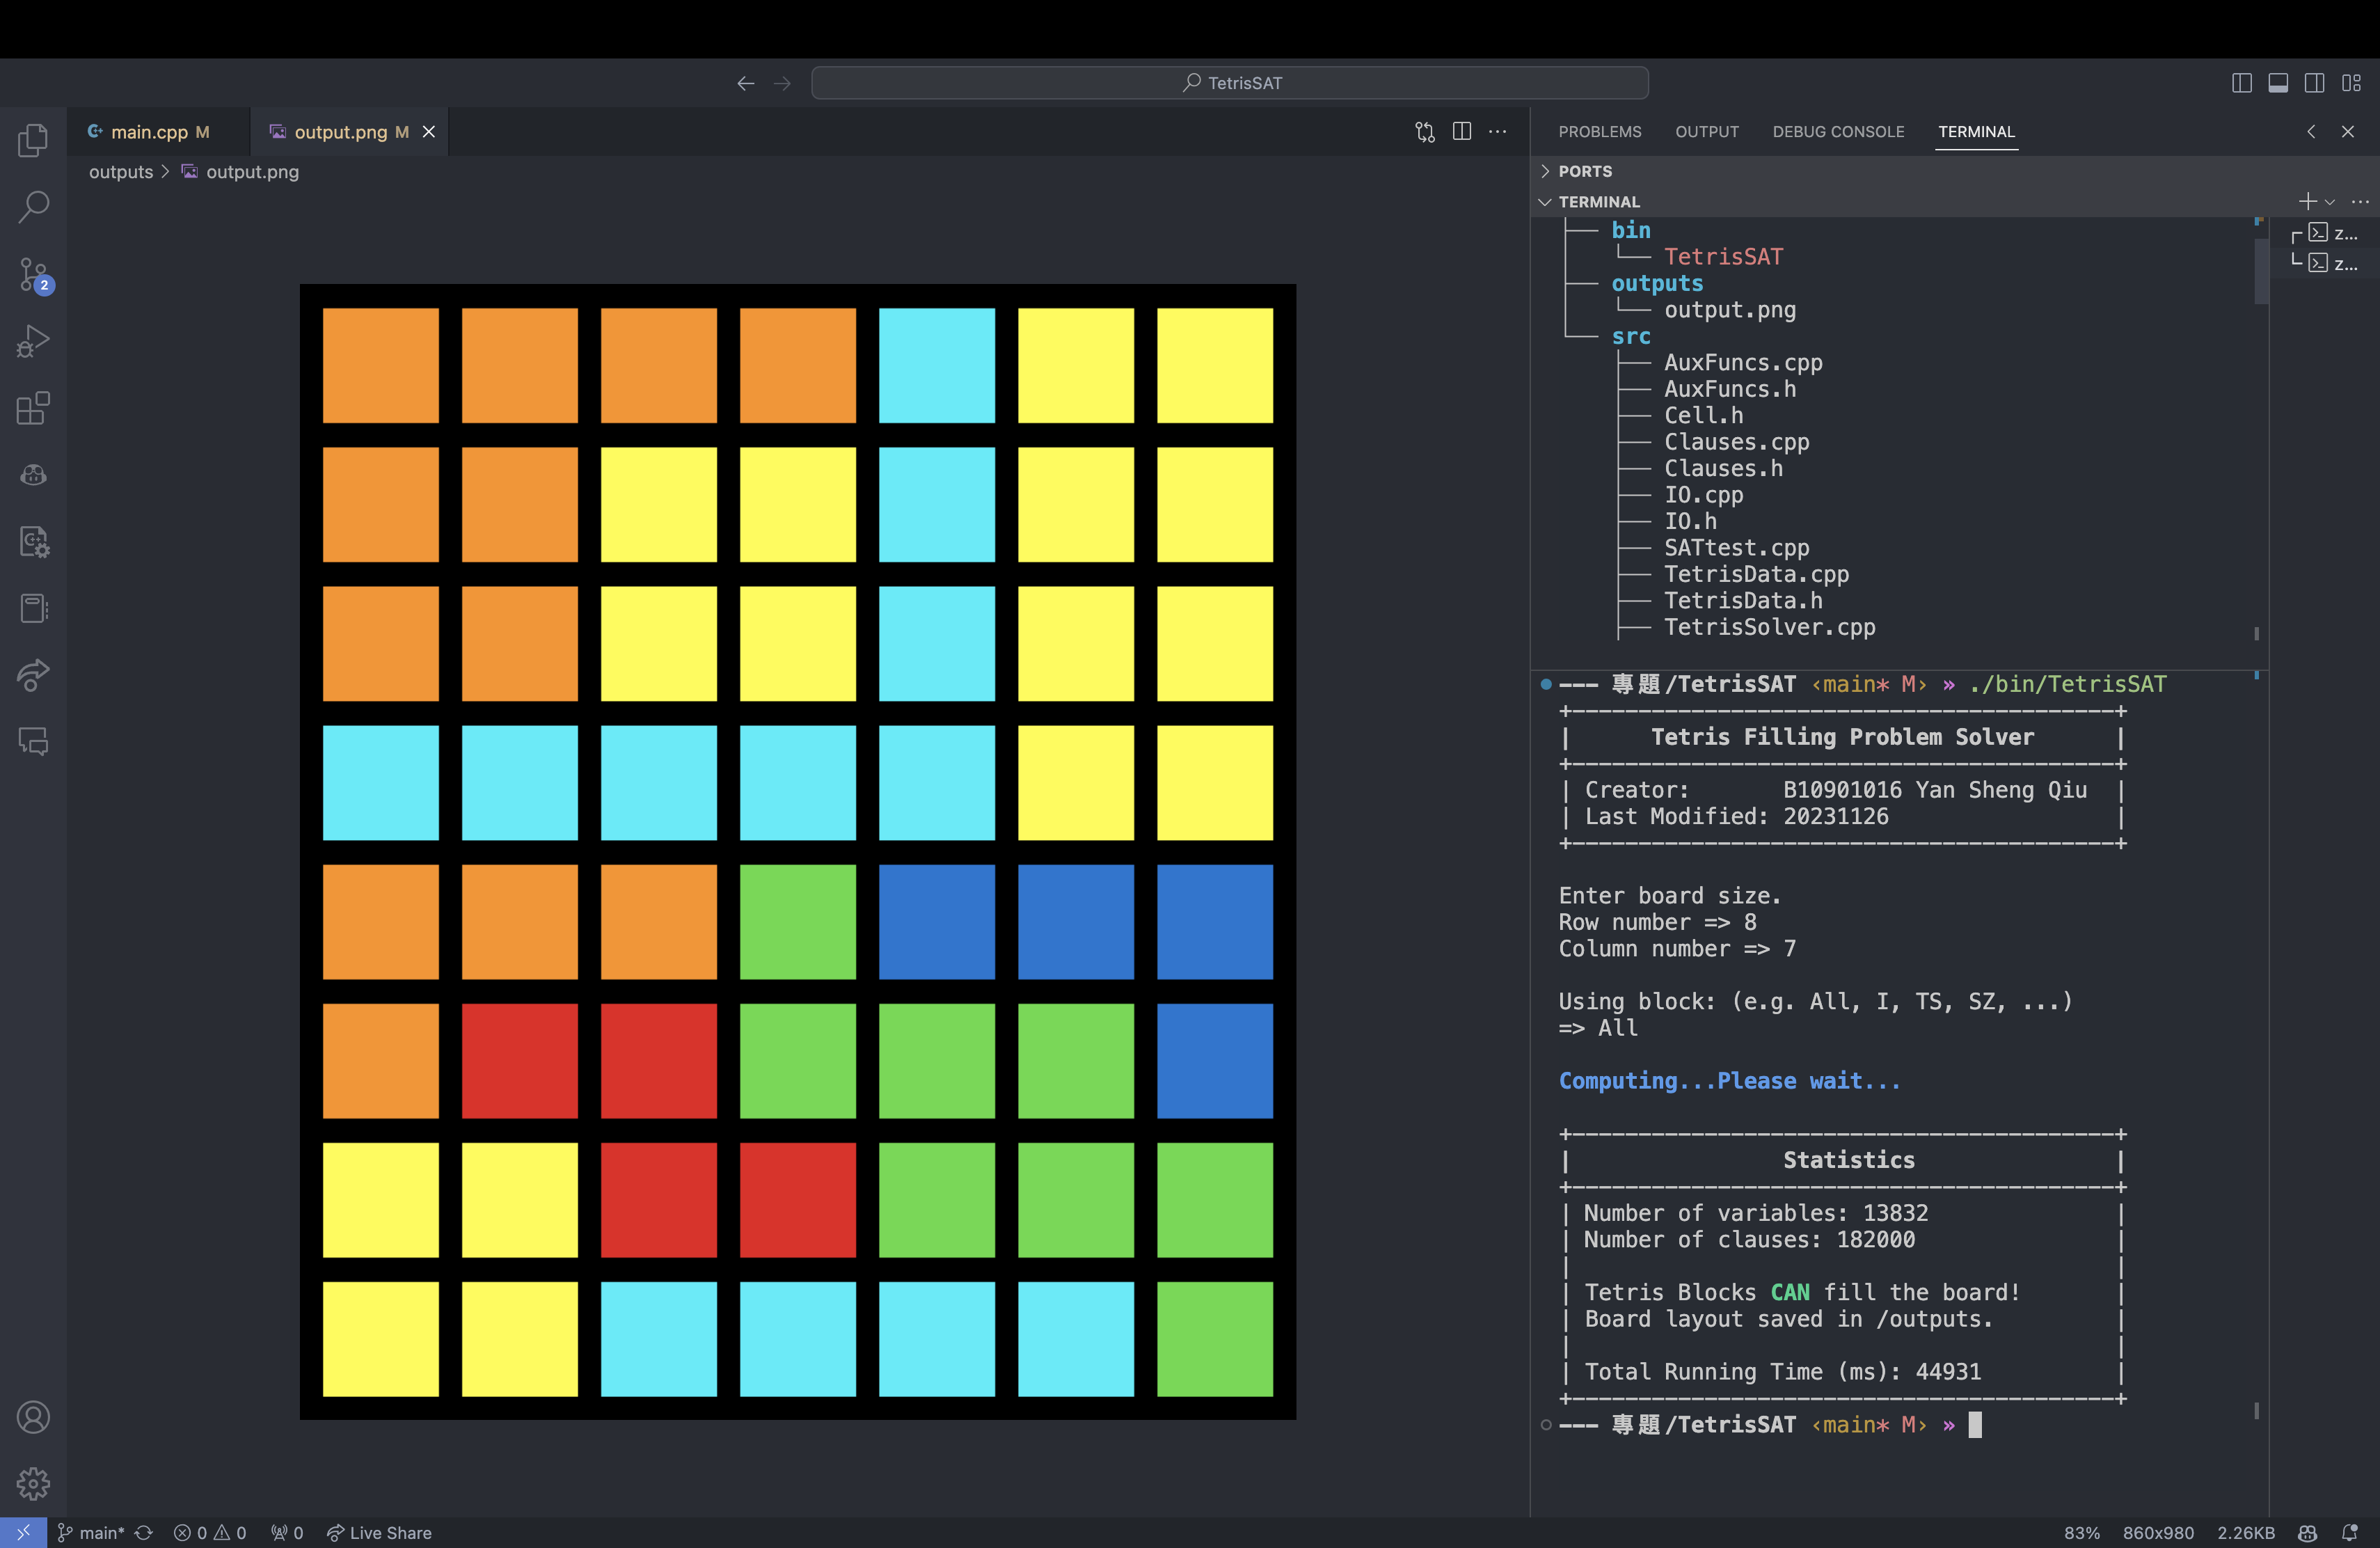
\includegraphics[width=0.8\textwidth]{Implementation.png}
            \caption{The solution of the $8\times 7$ board with the subset of blocks ``S, I, O, J, Z, T, L''.}
        \end{figure}
    \section{Experimental Results}
        % Give a table for the experimental results of different sizes of boards
        % m from 5 to 15, n from 5 to 15
        % m is placed on the row index, n is cloumn
        % The subset of blocks is ``S, I, O, J, Z, T, L''

        We use the subset of blocks ``S, I, O, J, Z, T, L'' to fill the boards with different sizes, from $5\times 5$ to $15\times 15$. The experimental results are shown in the table below, with the unit being microsenconds. Note if the total number of cells is not divisible by 4, we skip the measurement.

        \begin{table}[H]
            \centering
            \resizebox{0.9\textwidth}{!}{
                \begin{tabular}{|c|c|c|c|c|c|c|c|c|c|c|c|}
                    \hline
                    \diagbox{$m$}{$n$} & 5 & 6 & 7 & 8 & 9 & 10 & 11 & 12 & 13 & 14 & 15 \\
                    \hline
                    5 & - & - & - & 27750 & - & - & - & 51192 & - & - & - \\
                    6 & - & 22228 & - & 35526 & - & 49987 & - & 66766 & - & 67636 & - \\
                    7 & - & - & - & 44375 & - & - & - & 84220 & - & - & - \\
                    8 & 26002 & 35317 & 43987 & 53299 & 63883 & 77271 & 90097 & 102070 & 117240 & 133058 & 148925 \\
                    9 & - & - & - & 65382 & - & - & - & 126076 & - & - & -\\
                    10 & - & 50533 & - & 76884 & - & 108679 & - & 150066 & - & 201125 & -\\
                    11 & - & - & - & 92296 & - & - & - & 193371 & - & - & -\\
                    12 & 52284 & 69039 & 87036 & 105384 & 127987 & 149709 & 173821 & 203871 & 231921 & 259510 & 295343 \\
                    13 & - & - & - & 119340 & - & - & - & 230530 & - & - & - \\
                    14 & - & 88098 & - & 135169 & - & 191260 & - & 260026 & - & 339192 & -\\
                    15 & - & - & - & 152305 & - & - & - & 296178 & - & - & -\\
                    \hline
                \end{tabular}
            }
            \caption{The experimental results of different sizes of boards.}
        \end{table}
    \section{Observations}
        \begin{itemize}
            \item With all blocks used, all the boards with size $m\times n$ where $m\geq 5$ and $n\geq 5$ are completely fillable (Actually, intuitively, we can fill them with simple O blocks.).
            \item The experimental time compelixity is about $O(mn)$.
            \item There are always various kinds of blocks in the solution.
        \end{itemize}    
    \section{Future Work}
        \begin{itemize}
            \item The experimental time complexity is about $O(mn)$. Which conditions can be added to make the time complexity lower?
            \item Are there any other ways to model this problem?
            \item Can we fill the board with sufficient size (e.g. $m\geq 5$, $n\geq 5$) completely without O blocks and I blocks?
        \end{itemize}
\end{document}

% Delete trivial files
% rm *.aux *.log *.out *.synctex.gz

